\documentclass[uplatex,twocolumn]{jsarticle}
\renewcommand{\headfont}{\bfseries}
\renewcommand{\thesection}{\Roman{section}}
\renewcommand\thesubsection{\thesection.\Roman{subsection}}
\setlength{\columnsep}{3zw}
\setlength{\topmargin}{20mm}
\addtolength{\topmargin}{-1in}
\setlength{\oddsidemargin}{20mm}
\addtolength{\oddsidemargin}{-1in}
\setlength{\evensidemargin}{15mm}
\addtolength{\evensidemargin}{-1in}
\setlength{\textwidth}{170mm}
\setlength{\textheight}{254mm}
\setlength{\headsep}{0mm}
\setlength{\headheight}{0mm}
\setlength{\topskip}{0mm}
\usepackage[dvipdfmx]{graphicx}
\usepackage{float,nidanfloat,enumerate,amsmath}

\begin{document} 
\title{\large 研究計画書\\
\huge ルービックキューブとVRを活用した\\ 教育的効果に関する研究}
\author{千葉工業大学 先進工学部 未来ロボティクス学科\\
大川研究室 21C1034 苅込凌太郎\\
\small 指導教員 : 大川茂樹}
\date{2025年5月9日} 
\maketitle
\section{背景}
  %======================================================================================
  幼児教育において,パズルやゲームのような「遊び」は
  心身の成長を促すために重要である\cite{joy}.
  %======================================================================================
  Huda Fitriyaniらの研究\cite{puzzle}では5,6歳の児童に3Dパズル活動を実施させた.
  実際に使用されたパズルは家具や建物のミニチュアを模したパズルである.
  児童たちはこれらのパズルをバラバラの状態から,
  正しく組み立てるという活動をおこなった.
  研究の結果,こうしたパズル活動は空間認識や方向感覚の向上に寄与することが判明した.
  さらにルービックキューブのような複雑な立体パズルも,
  認知機能に好影響を与えることが分かっている.
  国立諏訪東京理科大学の研究\cite{rubik}によると,
  ルービックキューブを解くことで
  自頭力と深く関わるとされる前頭前野が活性化することが分かった.
  特に論理的思考力を司る左側の前頭前野に大きく影響することが判明した.
  ルービックキューブ学習後のテストの成績では,
  「応用力」・「思考の速さ」・「思考の深さ」において向上が見られた.
  \\\indent
  %======================================================================================
  このような教育的効果を持つ遊びを,
  より幅広く効果的に提供する手段として近年VR技術が注目されている
  \cite{全天球}\cite{授業実践}.
  VRは仮想空間で様々な現象を再現することが可能で,
  現実の制約にとらわれないオブジェクトや環境を作り出し,
  実際に見ることや体験できないことを立体的に提示することが可能である.
  %======================================================================================
  VR空間上に再現されたルービックキューブを解いた際に,
  現実のルービックキューブを解いた場合と同等の効果を得ることができたならば,
  新たな教材として活用できる可能性がある.
  %======================================================================================

\section{研究目的}
  ディスプレイ上やバーチャル空間上でパズルを解いても,
  実物のパズルを解いたときと同様な効果が得られるのかを検証する.

\newpage
\section{方法}
  \subsection{使用機器・開発環境}
    使用するヘッドマウントディスプレイ(HMD)はMeta Quest Proを採用する.
    このHMDは高解像度,広視野角に加えて優れた空間認識機能を備えているため,
    被験者に高度な没入体験を提供することができる.
    \\\indent
    開発環境はUnityエンジンを使用し,
    可能な限り実際のパズル体験に近づける.
    \\\indent

  \subsection{VR環境の構築}
  %======================================================================================
    ルービックキューブを解くことが目的であるため,
    環境は机のみが配置されている簡素な部屋をモデルとする.
    \\\indent
    一般的な3×3×3のルービックキューブは組み合わせが約430京通りあり,
    覚える手順も最低でも6から8個が必要である.
    一方で2×2×2のものは組み合わせが約370万通り,
    覚える手順も2から3個と少ない.
    揃えることがより容易である
    2×2×2のルービックキューブを採用する(図\ref{cube}).
    解法教示の表示などは行わない.
  %======================================================================================
    \begin{figure}[h]
      \begin{center}
        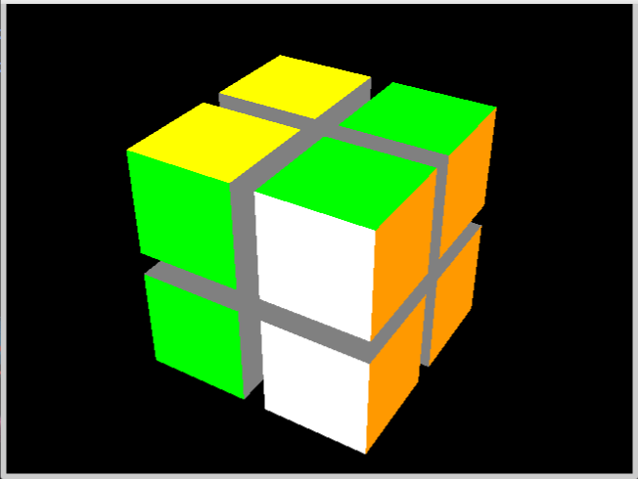
\includegraphics[width=50mm]{./images/cube.png}
        \caption{使用するルービックキューブ}\label{cube}
      \end{center}
    \end{figure}
  %======================================================================================

\newpage
\section{実験}
  本研究ではHuda Fitriyaniらの実験\cite{puzzle}に倣い,
  1日10回のパズル活動を実物で2週間,
  VR上で2週間の2回に分けて,計4週間行う.
  \\\indent
  被験者は小学校低学年20名で,10名ずつの2つのグループに分ける.
  グループAは1回目にVRで実験を行い,
  2回目は実物で行う.
  グループBは1回目に実物で行い,
  2回目はVRで行う(図\ref{flow}).
  %======================================================================================
  \begin{figure}[h]
    \begin{center}
      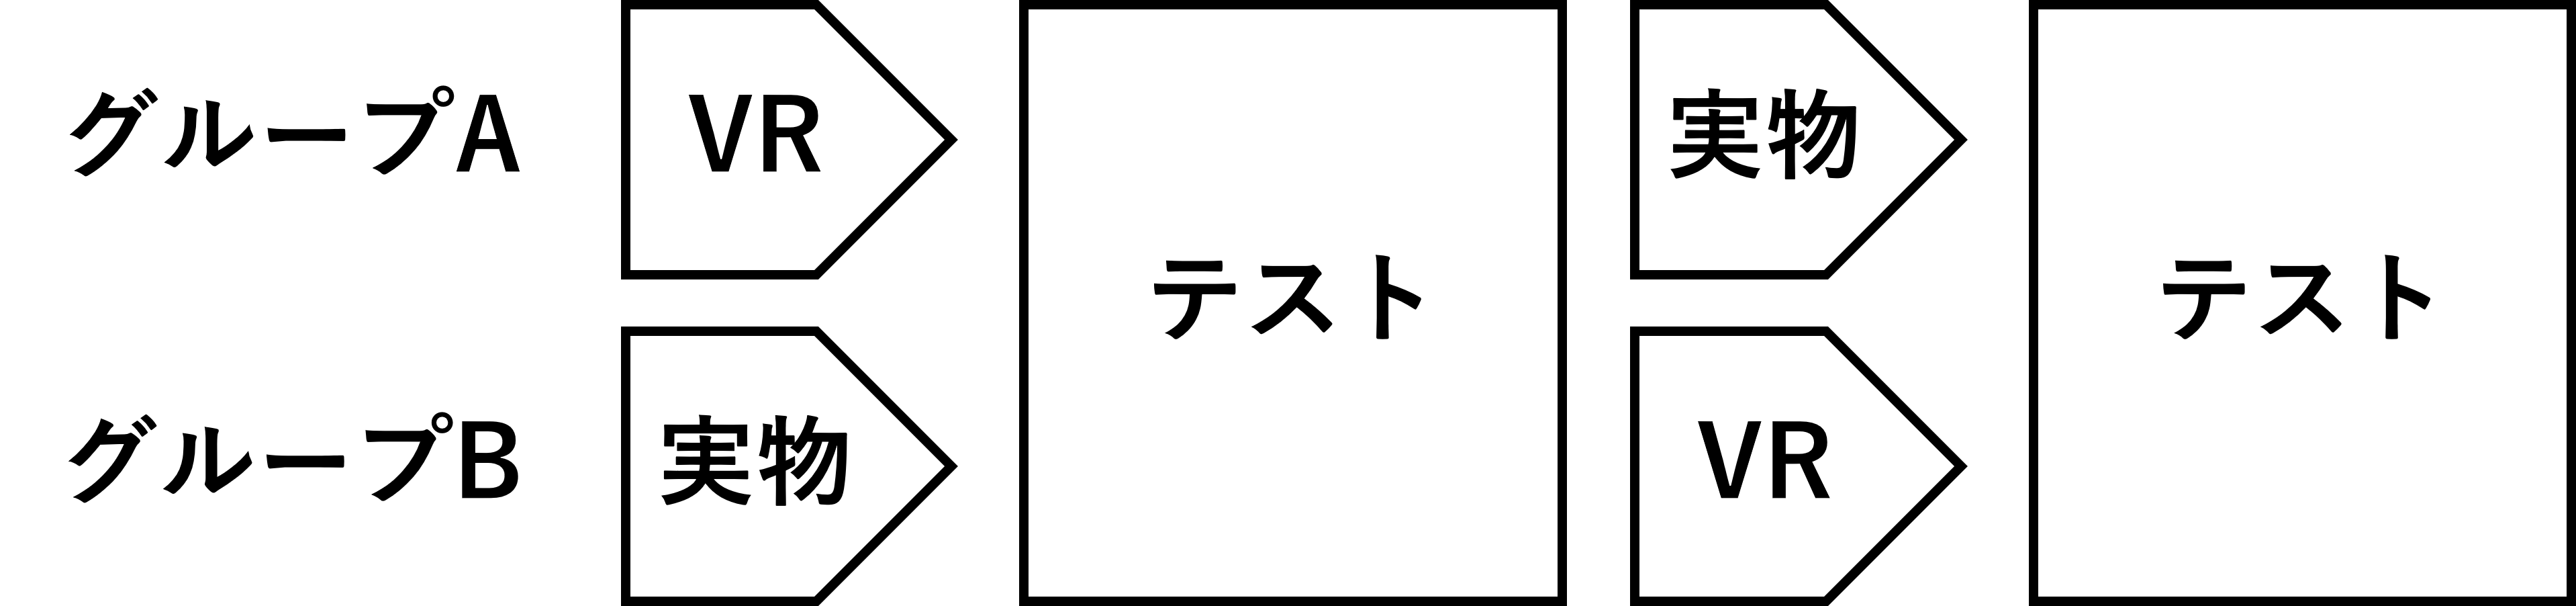
\includegraphics[width=80mm]{./images/experiment.png}
      \caption{実験の流れ}\label{flow}
    \end{center}
  \end{figure}
  %======================================================================================

\section{評価}
  \begin{enumerate}
    \item 切断面実形視テスト(MCT)\cite{MCT} \mbox{}\\
      透視図を使用して,
      立体の断面図から切り口の形状を正しく認識できるかを問うテスト.
      空間視覚化能力を評価する.
    \item N-back課題 \mbox{}\\
      ワーキングメモリは情報を一時的に保持しながら処理をする認知機能である.
      N-back課題はワーキングメモリの容量や処理能力を評価するために利用されている\cite{N-back}.
  \end{enumerate}

  評価は同グループの1回目と2回目の実験後のテスト結果の比較,
  1回目のグループAとグループBの比較と,
  2回目のグループAとグループBの比較の4回おこなう.

\section{スケジュール}
  \begin{description}
    \item M1 前期 :  VR環境の構築
    \item M1 後期 :  実験方法の検討
    \item M2 前期 :  実験,評価
    \item M2 後期 :  論文執筆 
  \end{description}

\section{期待される成果}

\section{入学後の抱負}
  入学後の抱負としては,
  継続的に発展させていけるような研究に取り組みたいと考えている.
  長期的な視点を持ち,着実に成果を積み重ねていける研究を目指したい.
  また得られた成果を社会に還元し,
  社会的課題の解決や人々の生活向上に貢献できるように努めたいと考える.
  個人としては,自ら主体的に課題を見つけ忍耐強く取り組むことで,
  研究者としての成長を遂げたいと考えている.

\begin{thebibliography}{9}
  \bibitem{puzzle}
    Huda Fitriyani,Neneng Tasu’ah,
    "The Use of Three Dimensional Puzzle as a Media to Improve Visual-Spatial Intelligence of Children Aged 5-6 Years Old",
    Indonesian Journal of Early Childhood Education Studies(2014)
  \bibitem{rubik}
    公立諏訪東京理科大学篠原研究室,
    "ルービックキューブ学習による脳活動への影響・創造性テスト成績の変化に関する調査",
    https://www.megahouse.co.jp/rubikcube/results/:w
  \bibitem{全天球} 
    瀬戸崎典夫,吉冨諒,岩崎勤,全炳徳,
    "全天球パノラマVRコンテンツを有する平和教育教材の開発",
    日本教育工学会論文誌(2015)
  \bibitem{授業実践}
    瀬戸崎典夫, 森田裕介,竹田仰,
    "ニーズ調査に基づいた多視点型VR教材の開発と授業実践",
    日本バーチャルリアリティ学会論文誌(2006)
  \bibitem{MCT}
    鈴木賢次郎,
    "認知図学事始め-切断面実形視テストによって評価される空間認識力-",
    図学研究,第33巻3号pp.5-12(1999)
  \bibitem{N-back}
    國見充展,松川順子,
    "N-back 課題を用いた視覚的ワーキングメモリの保持と処理の加齢変化",
    心理学研究,第80巻第2号pp.98-104(2009)
\end{thebibliography}

\end{document}
